\documentclass[tikz]{standalone}
\usepackage{tikz}
\usetikzlibrary{calc, angles, quotes}
\usetikzlibrary{intersections} % Necessário para achar pontos de cruzamento

\begin{document}

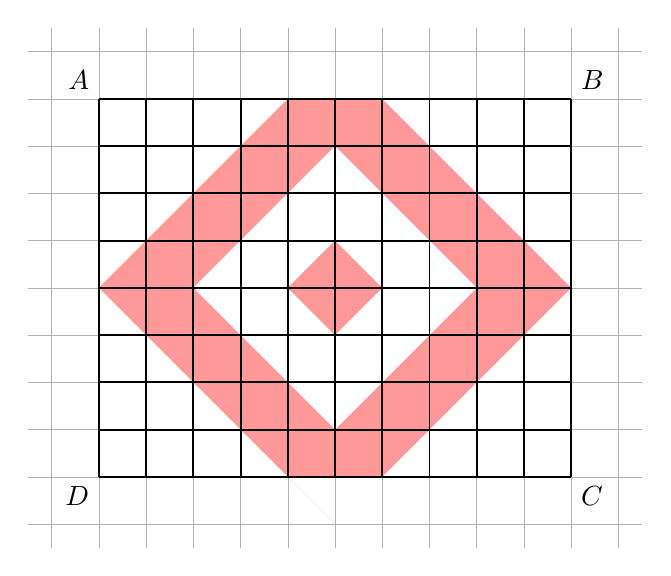
\begin{tikzpicture}[scale=.6]
 
  \draw[help lines,black!30] (-6.5,-5.5) grid (6.5,5.5);
   
  \def\x{5} \fill[red!40] (-5,0) -- (-1,4) -- (1,4) -- (5,0) -- (1,-4) -- (-1,-4) -- (0,-5);
  \def\x{3} \fill[white] (-\x,0) -- (0,\x) -- (\x,0) -- (0,-\x);
  \def\x{1} \fill[red!40] (-\x,0) -- (0,\x) -- (\x,0) -- (0,-\x);

  %\fill[red!40] (-1,0) -- (0,1) -- (1,0) -- (0,-1);
  \draw[help lines,line width=.7pt,black] (-5,-4) grid (5,4);

  \path (-5,4) node[above left] {$A$};
  \path ( 5,4) node[above right] {$B$};
  \path (5,-4) node[below right] {$C$};
  \path (-5,-4) node[below left] {$D$};

  
 
\end{tikzpicture}
\end{document}